\documentclass{llncs}
\pagestyle{plain}

\usepackage[n,advantage,operators,sets,adversary,landau,probability,notions,
logic,ff,mm,primitives,events,complexity,asymptotics,keys]{cryptocode}
%\usepackage{amssymb}
\usepackage{xspace}
%\usepackage[normalem]{ulem}
\usepackage{hyperref}

\title{Research Spike: Evaluation of Using a Single Mnemonic both
  for Cryptocurrency and Identity Wallets}
\author{}

% Custom shorthands for this paper
\definecolor{darkgreen}{rgb}{0.1,0.7,0.1}
\newcommand{\todo}[1]{{\colorbox{red}{\bf TODO:}\textcolor{red}{#1}}}
\newcommand{\doubt}[1]{{\colorbox{blue}
    {\textcolor{white}{\bf DOUBT:}}\textcolor{blue}{#1}}}
\newcommand{\response}[1]{{\colorbox{orange}{\bf RESPONSE:}
                                             \textcolor{orange}{#1}}}
\newcommand{\modified}[1]{{\textcolor{orange}{#1}}}
\newcommand{\commentwho}[2]{{\colorbox{darkgreen}{{\bf #1:}}
    \textcolor{darkgreen}{#2}}}
\newcommand{\comment}[1]{{\textcolor{orange}{\# #1}}}
%\newcommand{\note}[1]{{\colorbox{gray}{\bf NOTE:}\textcolor{gray} {#1}}}
\newcommand{\needcite}{[\colorbox{red}{?}]}
\newcommand{\figref}[1]{Fig. \ref{#1}}
\newcommand{\tabref}[1]{Table \ref{#1}}
\newcommand{\lstref}[1]{Listing \ref{#1}}
\newcommand{\secref}[1]{Section \ref{#1}}
\newcommand{\appref}[1]{Appendix \ref{#1}}
\newcommand{\defref}[1]{Definition \ref{#1}}

%\renewcommand{\qedsymbol}{$\blacksquare$}
\newcommand{\br}[1]{\ensuremath{\lbrack #1 \rbrack}}
\newcommand{\gen}[1]{\ensuremath{#1}}

\newcommand{\setind}[2]{\ensuremath{\set{#1}_{#2}}}

\mathchardef\mhyphen="2D
\def\suchthat{\ensuremath{s.t.}\xspace}

% General
\def\secpar{\ensuremath{1^\kappa}\xspace}
\def\Gen{\ensuremath{Gen}\xspace}
\def\Hash{\ensuremath{Hash}\xspace}
\def\tx{\ensuremath{tx}\xspace}
\def\getr{\ensuremath{\stackrel{\$}{\gets}}\xspace}
\def\arg{\ensuremath{arg}\xspace}
\def\msg{\ensuremath{m}\xspace}

% UC
\def\IdealF{\ensuremath{\mathcal{F}}\xspace}
\def\IdealG{\ensuremath{\mathcal{G}}\xspace}
\newcommand{\ucio}[1]{\ensuremath{\text{#1}}}
\newcommand{\uccmd}[1]{\ensuremath{\mathtt{#1}}}
\def\cmd{\ensuremath{cmd}\xspace}
\def\sid{\ensuremath{sid}\xspace}
\def\ssid{\ensuremath{ssid}\xspace}
\def\ucsend{\ucio{Send}\xspace}
\def\ucrecv{\ucio{Recv}\xspace}
\def\Sim{\ensuremath{\mathcal{S}}\xspace}
\def\Env{\ensuremath{\mathcal{E}}\xspace}
\def\Exec{\ensuremath{\text{EXEC}}}

% Signatures
\def\sig{\ensuremath{\sigma}\xspace}
\def\Sig{\ensuremath{\mathsf{S}}\xspace}
\def\IdealFSig{\ensuremath{\IdealF_{SIG}}\xspace}
\def\SIG{\ensuremath{\mathsf{SG}}\xspace}

% Hashes
\def\IdealGRO{\ensuremath{\IdealG_{RO}}\xspace}
\def\hashlist{\ensuremath{HL}\xspace}

% Key Types
\def\mpk{\ensuremath{mpk}\xspace}
\def\msk{\ensuremath{msk}\xspace}
\def\ipk{\ensuremath{ipk}\xspace}
\def\isk{\ensuremath{isk}\xspace}
\def\apk{\ensuremath{apk}\xspace}
\def\ask{\ensuremath{ask}\xspace}
\def\VK{\ensuremath{\mathsf{VK}}\xspace}

% Clock
\def\IdealGclock{\ensuremath{\IdealG_{clock}}\xspace}

% BB
\def\ldgLedger{\ensuremath{L}\xspace}
\def\IdealGledger{\ensuremath{\IdealG_{Ledger}}\xspace}
\def\IdealGdledger{\ensuremath{\IdealGledger^\delta}\xspace}
\def\ldgHonest{\ensuremath{H}\xspace}
\def\ldgMap{\ensuremath{M}\xspace}
\def\ldgState{\ensuremath{\Sigma}\xspace}
\def\ldgUtxo{\ensuremath{U}\xspace}
\def\ldgTx{\ensuremath{tx}\xspace}
\def\ldgBlock{\ensuremath{B}\xspace}
\def\ldgHead{\ensuremath{Head}\xspace}

% VDR
\def\VDR{\ensuremath{\mathsf{VDR}}\xspace}

% DIDs
\def\IdealGPKIDID{\ensuremath{\IdealG^{\P,\delta}_{\mathsf{PKIdvu}}}\xspace}
\def\did{\ensuremath{did}\xspace}
\def\DID{\ensuremath{\mathsf{DID}}\xspace}
\def\DIDCreate{\ensuremath{\DID.Create}\xspace}
\def\DIDRead{\ensuremath{\DID.Read}\xspace}
\def\DIDUpdate{\ensuremath{\DID.Update}\xspace}
\def\DIDReadLdg{\ensuremath{\mathsf{ParseLedger}}\xspace}
\def\didOp{\ensuremath{op}\xspace}
\def\didOP{\ensuremath{\mathsf{OP}}\xspace}
\def\didOWN{\ensuremath{\mathsf{OWN}}\xspace}
\def\typ{\ensuremath{t}\xspace}
\def\lbl{\ensuremath{l}\xspace}
\def\LBL{\ensuremath{L}\xspace}
\def\val{\ensuremath{v}\xspace}
\def\sval{\ensuremath{\mathbf{v}}\xspace}
\def\VAL{\ensuremath{V}\xspace}
\def\P{\ensuremath{\mathtt{P}}\xspace}
% \def\Pc{\ensuremath{\mathtt{P}_{\mathtt{C}}}\xspace}
% \def\Pu{\ensuremath{\mathtt{P}_{\mathtt{U}}}\xspace}
% \def\Pd{\ensuremath{\mathtt{P}_{\mathtt{D}}}\xspace}

% VCs
\def\VC{\ensuremath{\mathsf{VC}}\xspace}
\def\VCCreate{\ensuremath{\VC.Create}\xspace}
\def\VCPublish{\ensuremath{\VC.Publish}\xspace}
\def\VCRevoke{\ensuremath{\VC.Revoke}\xspace}
\def\VCShow{\ensuremath{\VC.Show}\xspace}
\def\VCVerify{\ensuremath{\VC.Verify}\xspace}

% Misc
\def\IdealFCA{\ensuremath{\IdealF_{CA}}\xspace}

% Atala
\def\RealPKIDIDAtala{\ensuremath{\Pi_{DID}^{Atala}}\xspace}
\def\phiDID{\ensuremath{\phi_{DID}}\xspace}
\def\MasterKey{\texttt{M}\xspace}
\def\AuthKey{\texttt{A}\xspace}
\def\CommKey{\texttt{C}\xspace}
\def\IssueKey{\texttt{I}\xspace}
\def\LMKL{\texttt{LMKL}\xspace}

%%% Local Variables: 
%%% mode: pdflatex
%%% TeX-master: "prism-protocol"
%%% End:


\begin{document}
\maketitle

\begin{abstract}
  \comment{\textbf{DISCLAIMER}: Please, keep in mind that this is a working
    draft. Its main use in its current state is to foster debate on the topics
    it deals with. Do not take anything written here as ground truth.}  
\end{abstract}

\section{Introduction}
\label{sec:introduction}

%%% Local Variables:
%%% mode: latex
%%% TeX-master: "single-mnemonic"
%%% End:

\section{An Overview of BIP32-based HD Wallets}
\label{sec:bip32}

Hierarchical Deterministic Wallets (HD wallets, for short) in the cryptocurrency
domain derive from the BIP32 specification%
\footnote{\url{https://github.com/bitcoin/bips/blob/master/bip-0032.mediawiki}.
  Last access, December 13th, 2021.}
The motivation behind creating this type of wallets is clear if one thinks about
how typical cryptocurrency systems work: each address is associated with a key
pair and, in order to achieve high security and privacy levels, it is best to
limit the reusage of addresses (thus, key pairs). Therefore, a too high number
of needed key pairs is quickly reached. If each key is generated independently
at random, management becomes too complex -- especially, if several devices
are expected to be synchronised. As a solution to this challenge, a hierachical
tree-based data structure was proposed, in which each parent node can be used to
derive multiple child nodes, deterministically. This approach seems also useful
to foster some sort of separation -- i.e., create sub-trees that are
(computationally) independent from one another, in the sense that a compromise
in one does not lead to a compromise in the other. Typically, the root node
of the tree is derived from a seed encoded as a mnemonic. BIP39%
\footnote{\url{https://github.com/bitcoin/bips/blob/master/bip-0039.mediawiki}.
  Last access, December 13th, 2021.} is the main specification for this purpose.

In this section, we give a brief overview of the BIP32 specification, and
provide a ``full path'' from mnemonic to key pair. To avoid repeating already
well documented processes, the overview will refer to the specifications when
appropriate.
%
In a final subsection, we will also overview how does all this apply to the
Cardano Lightwallet and Atala Prism cases.

\subsection{Main Specifications}

While the main specification is BIP32, it essentially gives the basic guidelines
to create HD wallets. To avoid ambiguity leading to incompatible
implementations, BIP43%
\footnote{\url{https://github.com/bitcoin/bips/blob/master/bip-0043.mediawiki}.
  Last access, December 13th, 2021.} and BIP44%
\footnote{\url{https://github.com/bitcoin/bips/blob/master/bip-0044.mediawiki}.
  Last access, December 13th, 2021.} specify how to organize HD wallets so
that the resulting tree structure enables the most common use cases (which, at
least initially, focus on the cryptocurrency scenario). In addition, the
specification that defines how to encode (pseudo-)random bitstrings as
mnemonic is given in BIP39.

\subsection{Main Concepts}

\begin{description}
\item[HD wallet tree structure.] HD wallets are organised as trees, where the
  root node is directly derived from the main seed (typically, a mnemonic-encoded
  random string). We denote the root level with level $0$, and all descendants
  with increasing numbers. A level other than the root level can have an
  arbitrary number of nodes.
\item[(Child) Index.] The child index just identifies how many childs can be (or
  have been) created before the current child, at the current depth of the tree.
  We assume $0$ to be the first index.
\item[Chaincode.] To introduce extra ``non-determinism'' in the way child keys
  are derived from parent keys, part of the pseudo-randomly derived data is
  used as key for pseudo-random derivations of lower levels. This part of the
  derived data is referred to as chaincode. We will denote the chaincode of the
  $j$-th node at level $i$ of the tree with $c_{i,j}$. This data should be kept
  secret; otherwise, entire subtrees can be compromised.
\item[Extended keys.] An extended public (resp. private) key is composed by the
  public (resp. private) key and the chaincode.  
\item[Hardened child keys.] A hardened child key can only be derived from the
  parent private key, and the parent key chaincode. 
\item[Non-hardened child keys.] A non-hardened child key can be derived both
  from the parent private and parent public key, and the parent key chaincode.
\end{description}

\paragraph{Hardened vs non-hardened child derivation.} Basically, child nodes
are derived as rerandomizations of their parent node private key. The
pseudo-random data used for rerandomization can be derived from the parent
private extended key, or from the parent public extended key. The former case is
referred to as hardened derivation, and the latter as non-hardened derivation.
In a nutshell, this means that hardened child keys (private or public) can only
be derived from their parent private key, but not from their parent public key.
Naturally, child private keys can only be derived from parent private keys.

For self-containedness, \figref{fig:childderivation} shows the different
algorithms to derive child keys from a parent keys, excluding some details. For
the full algorithms, we refer to BIP32.

\begin{figure}[ht!]
  \begin{minipage}[t]{0.55\textwidth}
    \procedure{$prv2HardChild$ \pccomment{Parent private key $\rightarrow$ $i$-th Child hardened key pair}}{
      \pcind I \gets HMAC(c_{par}, k_{par}, i) \\
      \pcind k^h \gets (k_{par} + Left(I)) \bmod n; K^h \gets k^hG; c^h \gets Right(I) \\
      \pcind \pcreturn (k^h,K^h,c^h) \\
    }
    \procedure{$prv2NonHardChild$ \pccomment{Parent private key $\rightarrow$ $i$-th Child non-hardened key pair}}{    
      \pcind I \gets HMAC(c_{par}, K_{par}, i) \\
      \pcind k^{nh} \gets (k_{par} + Left(I)) \bmod n; K^{nh} \gets k^{nh}G; c^{nh} \gets Right(I) \\
      \pcind \pcreturn (k^{nh},K^{nh},c^{nh}) \\      
    }
    \procedure{$pub2NonhardPubChild$ \pccomment{Parent public key $\rightarrow$ $i$-th Child non-hardened public key}}{      
      \pcind I \gets HMAC(c_{par}, K_{par}, i) \\
      \pcind K^{nh} \gets Left(I)G + K_{par}; c^{nh} \gets Right(I) \\
      \pcind \pcreturn (K^{nh},c^{nh}) 
    }    
  \end{minipage}
  \caption{Algorithms for child derivation. $k_{par},K_{par},c_{par}$ denote the
    parent's public key, private key, and chaincode, respectively. $k,K,c$
    denote the resulting child's private key, public key, and chaincode. $h$ or
    $nh$ superscripts denote hardened or non-hardened derivation. $Left$
    (resp. $Right$) divides a bitstring in two equal parts, and takes the left
    (resp. right) half. The result of both $Left$ and $Right$ can be interpreted
    as a scalar, and thus multipled by points in the elliptic curve, such as $G$,
    which is the base point, or public keys, which also are points in the
    curve.}
  \label{fig:childderivation}
\end{figure}

\paragraph{Isolation of HD wallet subtrees.} In the following section, we use
the concept of isolated and non-isolated subtrees. This is something that is
only indirectly mentioned in the BIPs and other related works, but which is of
crucial importance in order to limit the impact of compromised keys. Namely,
assume that a child key is derived in non-hardened mode. Then, if the extended
parent public key is leaked, as well as the private (non-extended) non-hardened
child key, it is possible to extract the parent private key -- and, therefore,
all the keys (private and public; hardened or not) that derive from it. If child
keys are derived in hardened mode, this does not apply. For the sake of clarity,
we illustrate the difference through the diagram in \figref{fig:isolation}.

\begin{figure}[ht!]
  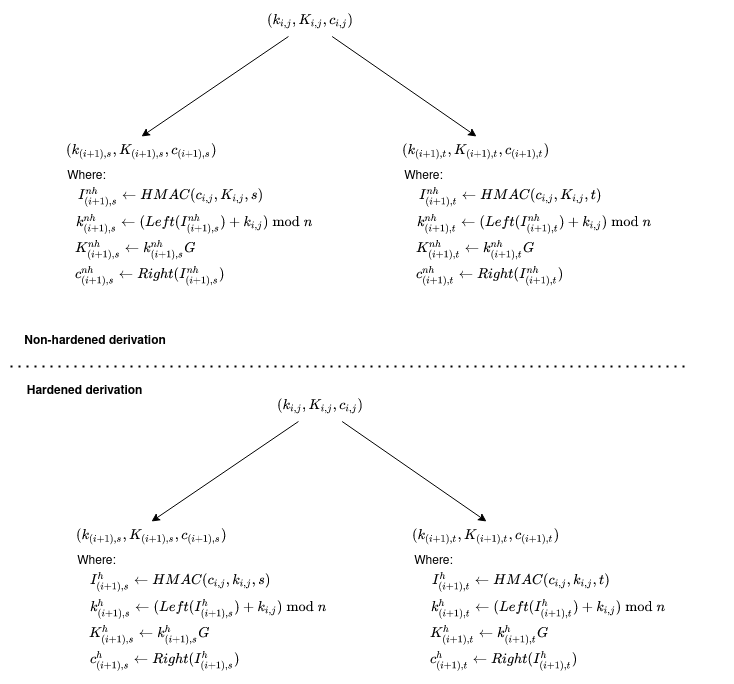
\includegraphics[width=\textwidth]{figures/child_derivation.png}
  \caption{Sub-tree isolation through hardened child derivation. $G$ is the
    base point of the underlying elliptic curve, and $n$ is the order of
    the associated group.}
  \label{fig:isolation}
\end{figure}

For instance, assume that the extended public key $(K_{i,j}, c_{i,j})$ is
compromised, along with its child private non-hardened key $k^{nh}_{(i+1),t}$.
Then, it is straightforward  to recompute the \emph{parent} private key
$k_{i,j}$ (independently on whether it was derived in hardened mode or not) as:
$k_{i,j} \leftarrow (K_{(i+1),t}^{nh} - Left(I_{(i+1),t}^{nh})) \bmod n$.
Obviously, given the parent private key $k_{i,j}$, it is straightforward to
derive all its descendants (hardened or not), as well as possibly and
recursively apply the same strategy, if the just recovered parent key was
derived in non-hardened mode.

\subsection{From Mnemonic to Key Pairs: High-level Overview}

The following description is based on BIP39 for the processing of mnemonics,
and BIP44 (which is a restriction of BIP43 and BIP32) for general structure of
an HD wallet, which we depict in \figref{fig:bip44-tree}.

\begin{figure}[ht!]
  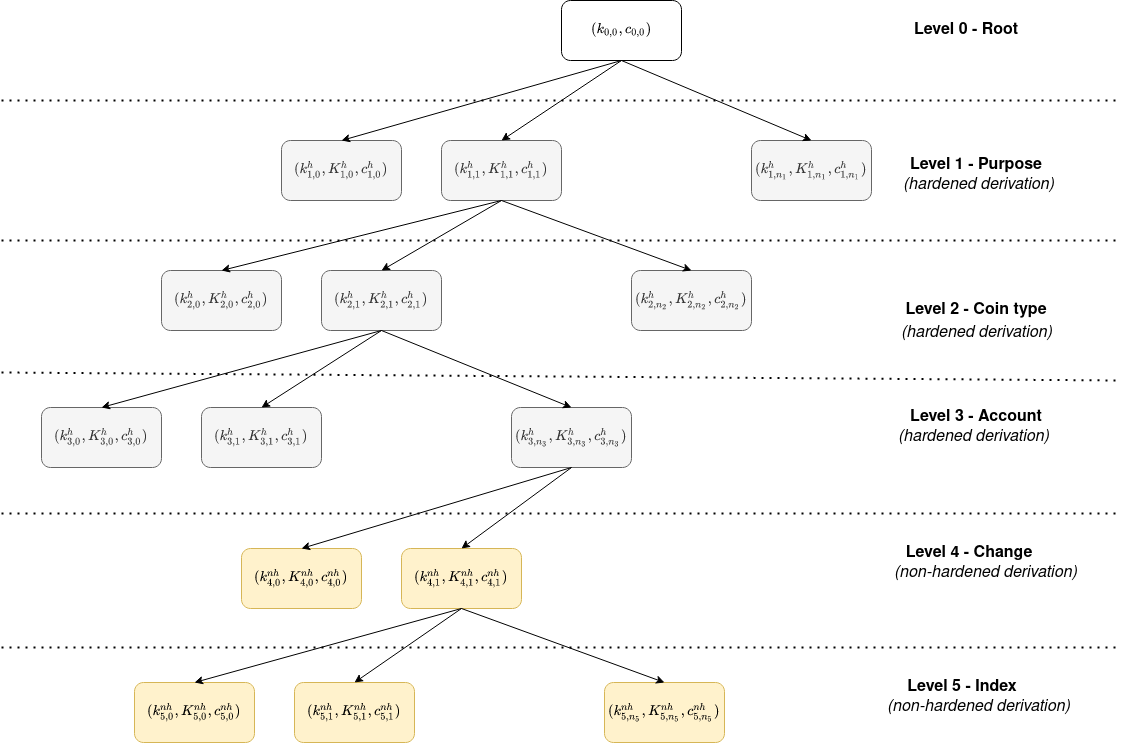
\includegraphics[width=\textwidth]{figures/bip44_tree.png}
  \caption{Basic tree structure of a BIP44-based HD wallet.}
  \label{fig:bip44-tree}
\end{figure}

\paragraph{From (pseudo-)random bitstrings to mnemonics, and back.} %
Mnemonics encode randomness in human-readable form. BIP39 is the main
specification for this. Roughly, between 128 and 256 random bits (in multiples
of 32) are generated, a checksum (the first few bits of a hash of these random
bits) is concatenated, and the result is divided in chunks of 11 bits. Each of
these chunks is used as index to a predefined dictionary of words. The result
is a mnemonic of 12 to 24 words. To convert from mnemonic to random bits, just
the inverse process has to be followed (verifying the checksum).

Given the mnemonic, it is converted back into a bitstring as just described.
Then, this bitstring is processed with an HMAC function, using the string
``Bitcoin seed'' as key based on SHA512 -- hence producing 512 bits of
output. The first 256 bits are set as master secret key, and the last 256 bits
as master chaincode (i.e., $k_{0,0}$ and $c_{0,0}$, in our previous notation).

\paragraph{Layer 1: \emph{isolated} subtrees per \texttt{purpose}} %
The first layer of a BIP44-compatible HD wallet is composed of up to $2^{31}$
nodes of hardened childs: i.e., layer 1 is composed of childs $(1,2^{31})$
to $(1,2^{62}-1)$, where the second element in the pair is the $i$ value used
in the child derivation processes, and denotes for what ``purpose'' the
descendant keys will be used -- this roughly translates to the system (e.g.,
Bitcoin, Cardano... or even non-blockchain systems, in theory).

Note that, being layer 1 computed in hardened mode, a private key compromise
of one node in layer 1 does not affect the master node, nor other layer 1
siblings. Hence, this is an ``isolated'' subtree, according to our terminology.

For BIP44-compatible wallets, the expected index is $44$. Cardano, since
the Shelley era, uses $1852$%
\footnote{\url{https://cips.cardano.org/cips/cip1852/}. Last access, December
  14th, 2021.}. Note that, since these are hardened indexes, the encoding
rules translate this into $1852+2^{31}$ (resp. $44+2^{31}$ for BIP44); see
BIP44 for more details.

\paragraph{Layer 2: \emph{isolated} subtrees per \texttt{coin type}} %
The second layer is again composed of up to $2^{31}$ nodes of hardened childs:
i.e., layer 2 is composed of childs $(2,2^{31})$ to $(2,2^{62}-1)$ per each child
node of layer 1. In theory, up to $2^{31}*2^{31}=2^{62}$ second-level nodes can
coexist in the same HD wallet. The aim of the second level is for any HD wallet
to be able to support multiple types of coins. E.g., so that the same mnemonic
can be used to derive key pairs for Bitcoin, Cardano, etc.

Note that, being layer 2 computed in hardened mode, a private key compromise
of one node in layer 2 does not affect its parent in layer 1, nor other layer 2
siblings. Hence, this is an ``isolated'' subtree, according to our terminology.

Although not mandatory, each coin is expected to have an assigned coin type
index. The complete list of reserved indexes is available in SLIP44%
\footnote{\url{https://github.com/satoshilabs/slips/blob/master/slip-0044.md}.
  Last access, December 14th, 2021.}.

\paragraph{Layer 3: \emph{isolated} subtrees per \texttt{account}} %
The third layer is again composed of up to $2^{31}$ nodes of hardened childs:
i.e., layer 3 is composed of childs $(3,2^{31})$ to $(3,2^{62}-1)$ per each child
node of layer 2. In theory, up to $2^{3*31}=2^{93}$ third-level nodes can
coexist in the same HD wallet. The aim of the third level is to allow the HD
wallet user to maintain many accounts per coin type. E.g., the same mnemonic
seed could be used for up to $2^{31}$ key pairs for Cardano addresses.

Again, note that being layer 3 computed in hardened mode, a private key compromise
of one node in layer 3 does not affect its parent in layer 2, nor other layer 3
siblings. Hence, this is an ``isolated'' subtree, according to our terminology.

\paragraph{Layer 4: \emph{non-isolated} subtrees per \texttt{change}}
According to BIP32, the fourth layer can be composed of up to  $2^{31}$ nodes of
non-hardened childs: i.e., layer 4 can be composed of childs $(4,0)$ to
$(4,2^{31}-1)$ per each child node of layer 3. However, in BIP44, only
non-hardened childs 0 and 1 are used: i.e., each node of layer 3 will only have
non-hardened childs $(4,0)$ and $(4,1)$. This layer is used to differentiate
whether the descendant nodes will be used as a change addresses, or not. I.e.,
child $(4,0)$ will \emph{not} be used for receiving change in payments, and
therefore is expected to be associated to an address that may be published
outside of the wallet; while child $(4,1)$ is expected to be used for receiving
change in payments.

Note that, since the 4th layer is not derived in hardened mode, if the private
key of the $(4,0)$ child of some layer 3 node is compromised along with the
extended public key of the node at layer 3, then the entire subtree of that
layer 3 node will be compromised (but not the subtrees of other layer 3 nodes,
as layer 3 is derived in hardened mode). That is, all the addresses (change or
not) of an specific account of some cryptocurrency, will be compromised.

\paragraph{Layer 5: \emph{non-isolated} final key pairs (\texttt{index})} %
The fifth and last layer is used to derive final key pairs. It can be composed
of up to $2^{31}$ non-hardened nodes: i.e., every change (and non-change) node
of level 4 may have level 5 childs from $(5,0)$ to $(5,2^{31}-1)$.

Note that, since layer 4 nodes are derived in non-hardened mode, if a layer 5
private key is compromised, as well as its parent extended public key of layer
4, then the whole layer 4 subtree will be compromised. Furthermore, if the
layer 3 extended public key from which the layer 4 parent derives is also
compromised, the entire account will be compromised too, as layer 4 is also
derived in non-hardened mode.

\paragraph{Notation.} It is frequent that the values used to derive keys in
the different layers are written in a short form like \texttt{m/a'/b'/c'/d'/e/f},
where \texttt{m} denotes the master seed (mnemonic); and each value between
bars is the number used to derive the key for the node at the corresponding
layer, where a tilded value denotes hardened derivation, and a non-tilded value
denotes non-hardened derivation. For instance, in the previous path, \texttt{a'}
denotes that the value \texttt{a} is used to derive, in hardened mode, the second
level of the path; or the value \texttt{f}  is used to derive, in non-hardened
mode, the last node in the path.

\subsection{Comments on a Recent Security Evaluation of BIP32 Wallets}

Very recently, \cite{def+21} was published in CCS'21, a major applied
cryptography and security conference. The paper builds on prior work from
2019 \cite{dfl19}, and analyses the security of BIP32-like wallets. For this purpose,
the authors first model and analyse (additively) re-randomizable signatures
built on ECDSA. They prove security, as long as every message is signed at
most once, at the cost of a security loss proportional to the number of
signature re-randomizations performed by the adversary\footnote{They also prove
  this security loss to be unavoidable with additive re-randomization, although
  I have not checked that proof.}. Then, they build a model for HD wallets,
and provide a generic construction using additively re-randomizable signatures.
The properties considered in this HD wallet model are unlinkability and
unforgeability (restricted to only one signature per message). The unlinkability
property expects that an adversary cannot distinguish (uncompromised) keys
derived from a non-hardened node, from keys derived from keys derived from an
independent master key. The unforgeability property is the usual one, excluding
the one message restriction (which seems reasonable, as long as new randomness
is included in every signed message); namely, the adversary should not be able
to create a valid signature under a hardened key that has not been compromised,
or a non-hardened key.

An interesting extension is mentioned, to achieve forward unlinkability in case
of compromise of non-hardened node public key and chaincode. Namely, if that
happens, the adversary will be able to derive the public extended keys for
all the subtree, which breaks unlinkability for the subtree. The proposal is to
keep a state along with every node. On every child derivation in the tree, the
state of the existing nodes is refreshed. Then, in case of compromise of a
node, the keys previously derived in subtrees of it are not affected (assuming
that previous states are securely erased).

Building on the proven security of the additively re-randomizable ECDSA, they
prove security of their generic construction, which now also depends on the
number of leaked hardened keys. Assuming that roughly $1\%$ of the total number
of (additively re-randomized) hardened keys are compromised, the estimated
security level for ECDSA of 256-bit keys (hence, 128-bit security) is 91-bit
security.

\paragraph{Discussion.} %
The model does seem to follow BIP32, but \textbf{assuming a hot/cold approach}.
Concretely, they assume that non-hardened secret keys are always kept in a cold
wallet, and therefore cannot be compromised. On the other hand, hardened secret
keys are assumed \emph{not} to be stored in cold wallets, and therefore can be
compromised (this is reflected in the model with corresponding oracles or lack
thereof). The underlying reasoning being that hardened derivation is used to
share keys with not fully trusted entities (e.g., employees in a company). Also,
hardened keys are assumed to be leafs (i.e., keys used directly for signing); or,
alternatively, roots of independent subtrees. Under this modelling, if the
partially trusted entity leaks the hardened key, this would only affect the
security of its subtree (if it exists), but certainly not siblings or ancestors.
However, this may not be fit for BIP44 wallets, where hardened derivation is
expected to be used directly for the first 3 layers, and the leaves are actually
computed with non-hardened derivation.

The property of forward unlinkability is interesting for identity-related
wallets.


%%% Local Variables:
%%% mode: latex
%%% TeX-master: "single-mnemonic"
%%% End:

\section{IO Ecosystem Specifics}
\label{sec:io}

\paragraph{Lightwallet.} HD wallets in Cardano are mostly BIP44-compatible
wallets, with the exception that the used elliptic curve is Ed25519,
instead of Secp256k1, like Bitcoin's BIP32 (and thus, BIP44). This
difference is marked by using index 1852 for hardened child derivation at
layer 1 (purpose level), as specified in CIP1852%
\footnote{\url{https://cips.cardano.org/cips/cip1852/}. Last access, December
  15th, 2021.}. Mnemonics in Cardano are composed by 24 words, and hence
encode 256-bit random bitstrings.

\paragraph{Atala.} HD wallets in Atala follow the same overall rules as in
BIP32. Specifically, the same distinction between hardened and non-hardened
child derivation rules are applied, as well as Secp256k1 as the elliptic curve,
wich ECDSA as digital signature scheme. However, Atala defines a different
tree structure, with the following layers, depicted also in \figref{fig:atalatree}:

\begin{description}
\item[Layer 0: Root.] Encoded as/derived from a 12-word mnemonic.
\item[Layer 1: DID Number.] Obtained by hardened child derivation from the root.
  Each node in this level corresponds to a different DID.
\item[Layer 2: Key Type.]  Obtained by hardened child derivation from a layer 1
  node. Currently, the Atala specification defines four types of keys: master
  keys, issuing keys, communication keys, and authentication keys.
\item[Layer 3: Index.] Obtained by hardened child derivation from a layer 2 node.
  Each layer 2 node may have up to $2^{31}$ child nodes, which are the leaves of
  the tree.
\end{description}

See the key derivation document for details%
\footnote{\url{https://github.com/input-output-hk/atala-prism/blob/master/prism-backend/docs/protocol/key-derivation.md}. Last access December 15th, 2021. \textbf{WARNING!
    Internal link!}}. Mnemonics in Atala are composed by 12 words, and hence
encode 256-bit random bitstrings.

\begin{figure}[ht]
  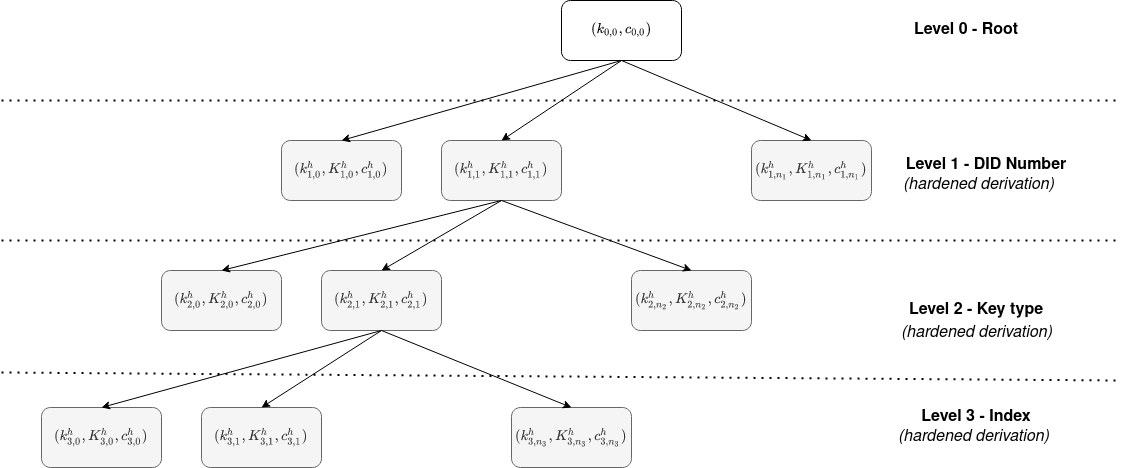
\includegraphics[width=\textwidth]{figures/atala_tree.png}
  \caption{Atala tree derivation structure.}
  \label{fig:atalatree}
\end{figure}

\paragraph{Note on the different cryptographic choices.} As stated, Cardano's
Lightwallet CIP1852 follows a variation of BIP44 where the chosen singing
algorithm is EdDSA, which uses Ed25519 as elliptic curve; whereas Atala builds
from BIP32, thus employs ECDSA with a secp256k1 curve. The reason behind this
difference seems just circumstancial, and due to the fact that Atala started to
build from a different specification. From a cryptographic point of view, it is
possible to unify under the same curve, or to stick to different ones. In the
latter case, however, we must make sure that domain separation is correctly
done: i.e., even if having a sort of unified wallet derived from the same
mnemonic, it should not be possible to generate the same key to be used for
payment purposes and identity purposes. More detail on this is given in
\secref{ssec:unification}.

Other than the previous, either choice seems to have its pros and cons. On the
one hand, having both Cardano and Atala use the same curve would make it
possible to benefit from joint development efforts. Also, it would avoid
pitfalls such as using the same key in different curves, which can lead to
security issues as described next (however, this can also be avoided with proper
domain separation). Also, Edwards curves (such as Ed25519) are, at least in
theory, more efficient. On the other hand, Secp256k1 is an standardized curve,
which has seen more implementation and optimization effort. This means that the
better theoretical efficiency of Ed25519 may somehow ``mitigated'' by more
efficient implementations in Secp256k1. Also, Secp256k1 probably has more
availability of implementations in different programming languages. In any case,
this is something that needs to be considered by the development/engineering
teams.

\paragraph{Related effots.} There seems to be an effort to analyse the security
of wallets that manage addresses combining payment and staking keys \cite{kkl20}.
These wallets are referred to as PoS wallets. The paper identifies a series of
malleability attacks, depending on how the addresses are derived from the
associated staking and payment keys. A core wallet functionality is proposed,
and a base protocol realizing that functionality is given. While the proposal
seems to be somehow compatible with BIP44 wallets, the proposal seems to be
somehow orthogonal to the way keys are derived -- instead, they focus on how
to generate addresses, and check that produced/received addresses are correct.

\subsection{Aspects to consider before unification}
\label{ssec:unification}

Next, we emphasize some concrete topics that would need to be considered
from an implementation/software-design point of view, prior to making
Atala and Cardano keys to be derived from a single mnemonic.

\paragraph{Domain separation when different cryptosystems is
  necessary.} %
As mentioned, Cardano uses EdDSA (which is based on Ed25519 curve),
while Atala uses ECDSA with Secp256k1. It is \emph{not} a good idea%
\footnote{I have not been able to find a paper that describes
  some concrete related attack or gives some impossibility result for
  proving security under this circumstance but, at the least, it seems to
  be folklore knowledge. See Lindell's answer at
  \url{https://crypto.stackexchange.com/a/54666/52362} for instance.
  \cite{dlp12+,thorm21} seem good references to study this topic further, if
  needed.} to use the same key in different cryptosystems, nor for different
curves, even though ``structurally'' it may be possible (e.g., in EdDSA and
ECDSA, private keys are 32-byte random numbers). However, this is easily
avoidable by ensuring domain separation in the key derivation functions that
are applied on the common seed. This is an important concern on its own; yet,
it should be addressed natively through the considerations in the next
paragraph.

\paragraph{Ensure a correct hierarchical key derivation strategy.} %
We need to take into account what specific usage we expect from the wallets
and, from there, define hierarchical derivation rules that ensure security
without disabling current utility. Related to the previous paragraph, we should
make sure that keys that are aimed to be used in different
cryptosystems, are derived in separate tree branches that ensure domain
separation. Or, since the Atala derivation path is shorter, than no Atala
derivation path can be a prefix of a Cardano derivation path. For instance,
according to the current specification, the derivation path
\texttt{m/1852'/1815'/0'} corresponds to account \texttt{0'} for Ada coins in
CIP1852-compliant Cardano wallets. In Atala, \texttt{1852'} could be a valid
DID number and, while \texttt{1815'} is currently not a valid key type, if,
in the future it becomes so, then \texttt{m/1852'/1815'/0'} would be a valid
derivation path in both Atala and Cardano -- which could open an attack vector.
An easy fix would be to concatenate the master seed with some value \texttt{C}
in Cardano, and some distinct value \texttt{A} in Atala. The derivation paths would
become \texttt{Cm'/1852'/1815'/...} in Cardano, and \texttt{Am'/...} in Atala
-- hence, domain separation would be ensured. Probably, many other alternatives
exist, more suitable from an engineering perspective (e.g., assigning Atala its
own \texttt{purpose} level in BIP44 wallets). But, whatever option is followed,
domain separation should be ensured.

\paragraph{On the mnemonic length.} %
Atala uses 12-word mnemonics to encode the master seed from which all keys are
derived, while Cardano uses 24 words. According to BIP39, 12 words encode 128-bits
seeds, and 24 words encode 256-bit seeds. These entropy bits are then subject to
the extract-and-expand approach of the HKDF used in BIP32 to produce pseudoranom
bits that are computationally indistinguishable from true random numbers%
\footnote{Note: only 256 of these bits are used to produce the final keys.}.
The keys used by both Atala (for ECDSA), and Cardano (for EdDSA), are thus
securely derived pseudorandom keys of 256 bits. For keys of 256 bits, both ECDSA
and EdDSA are expected to provide 128 bits of security against unforgeability
attacks. Given this, and assuming (like \cite{def+21} does) that some keys
will be compromised, there are two ways to attack a wallet: by breaking
security of the HKDF used to derive the keys; or by breaking security of
the wallet construction itself. Given this, on the one hand, in \cite{def+21}%
\footnote{Important! Note that \cite{def+21} is defined for ECDSA-based BIP32
  wallets with a structure slightly different from BIP44 wallets. Hence, its
  results may not translate to our setting -- and of course, neither to
  EdDSA-based BIP44 wallets.}, security of BIP32 wallets against unforgeability
is estimated to have a security loss of 37 bits over the underlying digital
signature scheme (under somewhat arbitrary estimations for
a typical setting, like leaking about $1\%$ of roughly $2^{20}$ produced
keys). For 256-bit ECDSA keys, this translates to 91 bits of security.
On the other hand, even for 128-bit seeds (thus, with entropy at most
128), breaking the security of the HMAC-based HKDF construction (that would
seem to affect the unlinkability property of BIP32 wallets, rather than their
unforgeability) would be harder than breaking the unforgeability property of
the BIP32 wallet, as per the results in \cite{kraw10}\footnote{According to the
  analysis in \cite{kraw10}, the outputs of HMAC-based HKDFs are roughly
  $q2^{-m}$-close to uniform, where $q$ in our setting would be $2^{20}$ as per
  \cite{def+21}, and $m$ is the min-entropy of the randomness source (our
  mnemonic). Hence, for seeds (mnemonics) of 128 bits of entropy, we can still
  expect the outputs to be $\sim 2^{-100}$-close to uniform.}. Given this, and
lacking a more detailed analysis, seeds of 12 words would appear to be enough
for security, strictly speaking. However, taking into account that we are
aiming to combine two wallets into one, it does not seem logical to reduce the
overall security of the wallet that uses 24-word mnemonics, as the unified
wallet will use the same mnemonic to produce even more keys than what it
was producing before. Therefore, it seems advisable to increase the mnemonic
length of Atala to 24 words, rather than reducing the length of Cardano to
12 words.

%%% Local Variables:
%%% mode: latex
%%% TeX-master: "single-mnemonic"
%%% End:

\section{Discussion}
\label{sec:discussion}

From a theoretical point of view, it seems very reasonable to derive all
keys, even for different purposes (payments, staking, or identities) from
the same mnemonic. However, there are some aspects that may need careful
consideration, as they may have impact in the overall security and privacy
properties of the wallet (and related systems).

\paragraph{Domain separation when different cryptosystems are
  necessary.} %
As mentioned, Cardano uses EdDSA (i.e., it is based on Ed25519 curve),
while Atala uses ECDSA with Secp256k1. It is \emph{not} a good idea%
\footnote{I have not been able to find a concrete paper that describes
  some concrete related attack or gives some impossibility result for
  proving security under this circumstance but, at the least, it seems to
  be folklore knowledge. See Lindell's answer at
  \url{https://crypto.stackexchange.com/a/54666/52362} for instance.
  \cite{dlp12+,thorm21} seem good references to study this topic further, if
  needed.} to use the same key for different cryptosystems, nor for different
curves, even though ``structurally'' it may be possible (e.g., in EdDSA and
ECDSA, private keys are 32-byte random numbers). However, this is easily
avoidable by ensuring domain separation in the key derivation functions that
are applied on the common seed. Since this would be handled by the 

\paragraph{Ensure a correct hierarchical key derivation strategy.} %
We need to take into account what specific usage we expect from the wallets
and, from there, define hierarchical derivation rules that ensure a correct
separation. For instance, related to the previous paragraph, we should make
sure that keys that are aimed to be used in different cryptosystems, are
derived in tree branches that ensure domain separation (just using a
different \texttt{purpose} branch, or \texttt{coin type} branch, would probably
be enough). Similarly, one needs to consider if specific subtrees are expected
to be used in an standalone manner, even probably by different (but related)
entities. For instance, different faculties of a university may need to maintain
their own subrees for the sake of efficiency (i.e., each one independently
deriving keys as needed). But then, compromises to one of them should not
affect the other. Again, this can be easily achieved using hardened
derivation in BIP44 slang (e.g., at the \texttt{account} level). From this
point of view, a formalization along the lines of \cite{def+21} would be
desirable, but the one given there is probably too strict (as, for instance,
it assumes that hardened nodes are leaves of the tree, and secret key
compromise of non-hardened nodes, is not possible.)

\paragraph{Malleability considerations when combining multiple
  attributes into one address.} %
Are the keys for the different purposes going to be used \emph{only} in a
standalone manner? Or, rather, it can be expected that they are somehow
encoded and distributed jointly? The latter seems to be the case for PoS
wallets, which are expected to be used in the Cardano ecosystem. As pointed
out by \cite{kkl20}, naive encoding of keys with different purposes, into
a single address, may enable certain (malleability) attacks.

\paragraph{Careful consideration of extra security properties.} %
The main related work analysed so far\footnote{BIP32, BIP44, \cite{def+21}
  and, partially, \cite{kkl20}.} analyses the security of either BIP44
wallets, or PoS wallets. The introduction of identity-related (frequently
associated to actual people) data may require additional properties, only
mentioned in these works (or not considered, as in the BIPs). For instance,
some sort of forward security will be very desirable. While, for the case of
payments or staking, the impact of a compromise (either of a leaf node --
i.e., a key -- or a complete subtree) can be mitigated by prompt detection
and transfer of funds to an uncompromised address, this may be harder for
keys representing in some way real world identities. Most probably, the
latter will frequently be long-lived keys, that also can, in turn, be used
to issue further identities (e.g., as in the case of identity providers).
Thus, the consequences of a compromise may be more cumbersome to address
(re-issuing credentials, distributing revocation lists, etc.) and,
consequently, it seems desirable to look for constructions that give some
sort of guarantee about the security of keys produced at time $t' < t$, if a
compromise happens at time $t$.

Also, it cannot be discarded that further desirable privacy or security
properties arise, as we get more familiar with the targetted use cases.
  
\subsection{Further related work}

There seems to be a large body of related research, which is specially
growing lately (probably, due to the rise of cryptocurrencies). Here,
I just include some of the main references I've come across for
self-bookkeeping (besides \cite{kkl20} and \cite{def+21}, already
mentioned in earlier sections). Note that they, in turn, include references
to further related work.

\begin{itemize}
\item ``Arcula: A Secure Hierarchical Deterministic Wallet for Multi-asset
  Blockchains'', \cite{lfa20}.
\item ``Simple, Efficient and Strongly KI-Secure Hierarchical Key Assignment
  Schemes'', \cite{fpp13}.
\item ``A Formal Treatment of Deterministic Wallets'', \cite{dfl19}.
\end{itemize}

%%% Local Variables:
%%% mode: latex
%%% TeX-master: "single-mnemonic"
%%% End:

%\section{Conclusion}
\label{sec:conclusion}

\comment{This section is just a placeholder for now...}

%%% Local Variables:
%%% mode: latex
%%% TeX-master: "uas"
%%% End:


\bibliographystyle{splncs04}
\bibliography{single-mnemonic}

\end{document}

%%% Local Variables:
%%% mode: latex
%%% TeX-master: single-mnemonic
%%% End:
